\chapter{Results}
\label{chap:Results}

In this chapter, we will present the results obtained from our project. 
Firstly, we will demonstrate how the automation routine enhanced the research experiments. 
Next, we will discuss the validation of the classification results. 
Finally, we will showcase the performance of the implemented controller algorithms.

\section{Automation routine}
\label{sec:automation_routine}

The automated experiment routine is capable of acquiring a significantly more precise and extensive amount of data than what can be achieved by a human. 
With the save data by streaming in saving thread\ref{subsec:save_thread}, we achieved less program memory during the experiment and, specially, safety for not losing the data in case the program fail during an experiment.

Also, most power supplies rely on manual potentiometer adjustment to select the set point, which results in imprecise potential selection by a person. 
Moreover, manual adjustment takes some time to achieve the desired voltage. 
By running a computer routine that automatically sends commands to the power supply and pump machine we can achieve faster and more reliable experiment data points.

The visual interface for the user, seen in figures \ref{fig:multi_class_exp1} and \ref{fig:multi_class_exp}, shows all the important sensor data and signal analysis that can be interesting to the operator in real time.

\begin{figure}[H]
    \center
    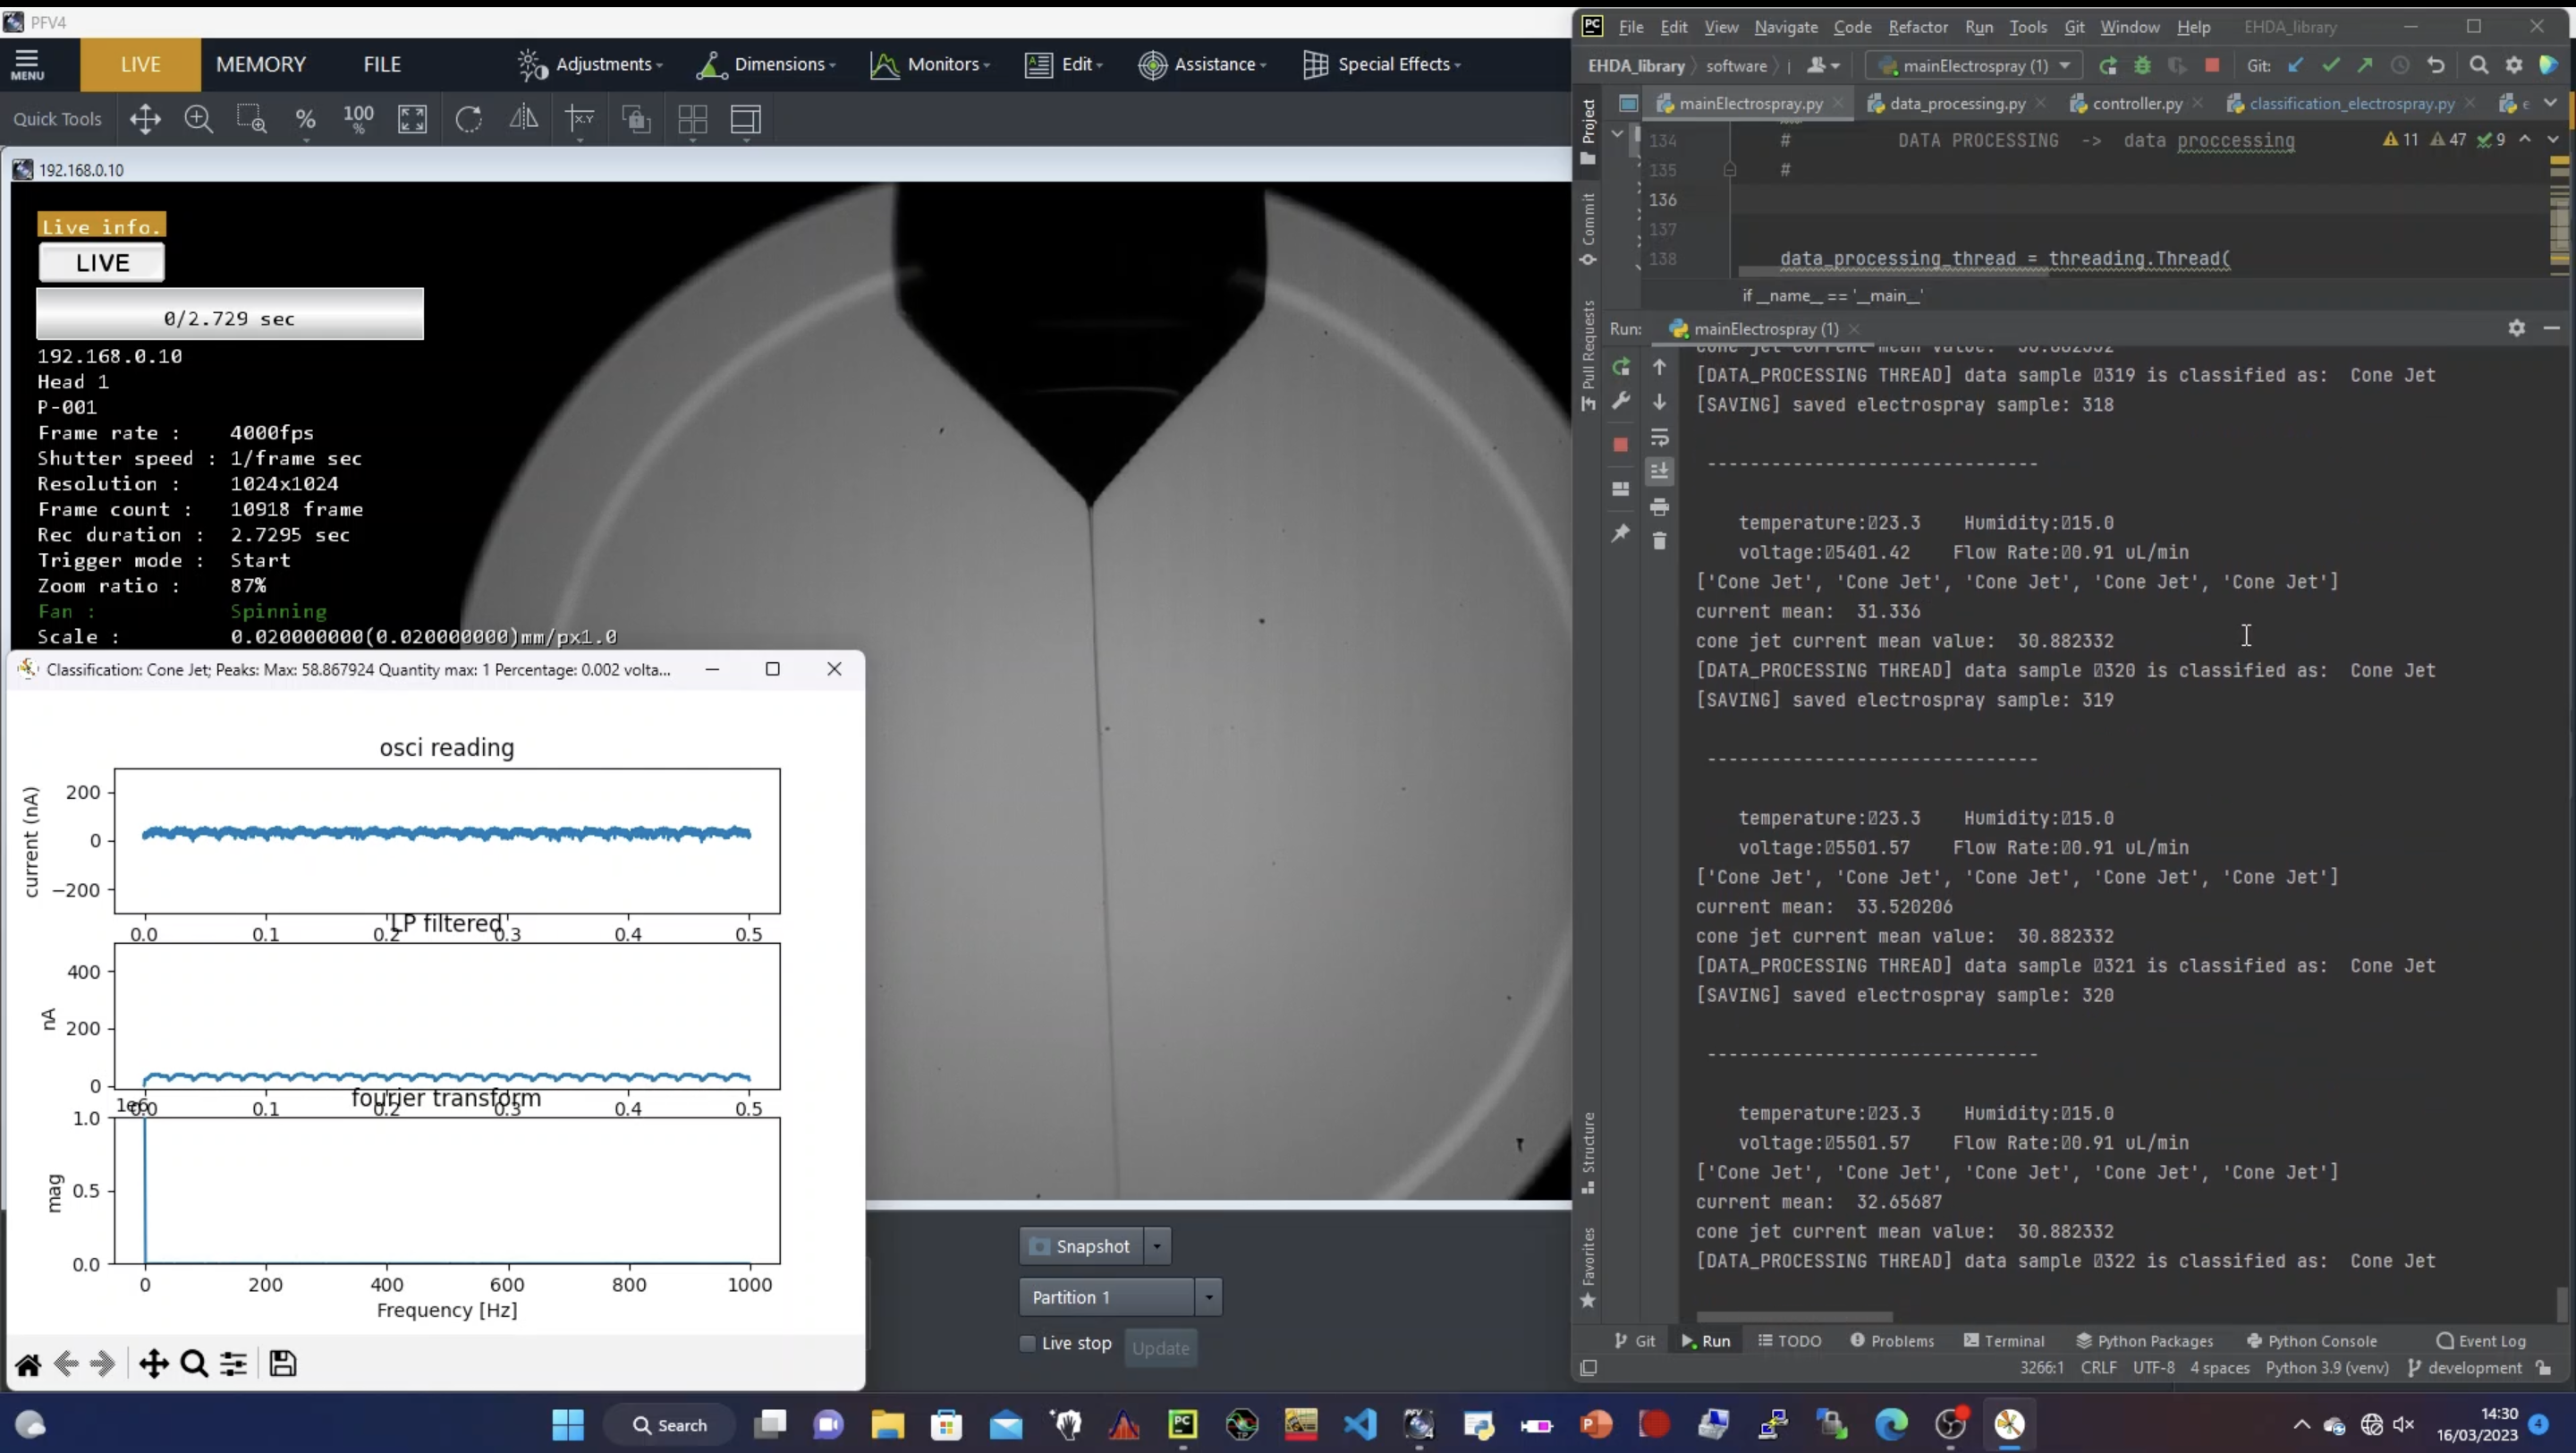
\includegraphics[width=16cm]{Figuras/19:03/axs1.png}
    \caption{Print screen of the window shows user interface during the experiment.
        We can see the image generated by the camera in the background.
        The routine code running in pycharm software on the right side.
        And also real time signal plottings of the current data on the left side.}
        \label{fig:multi_class_exp1}
\end{figure}


\begin{figure}[H]
    \center
    {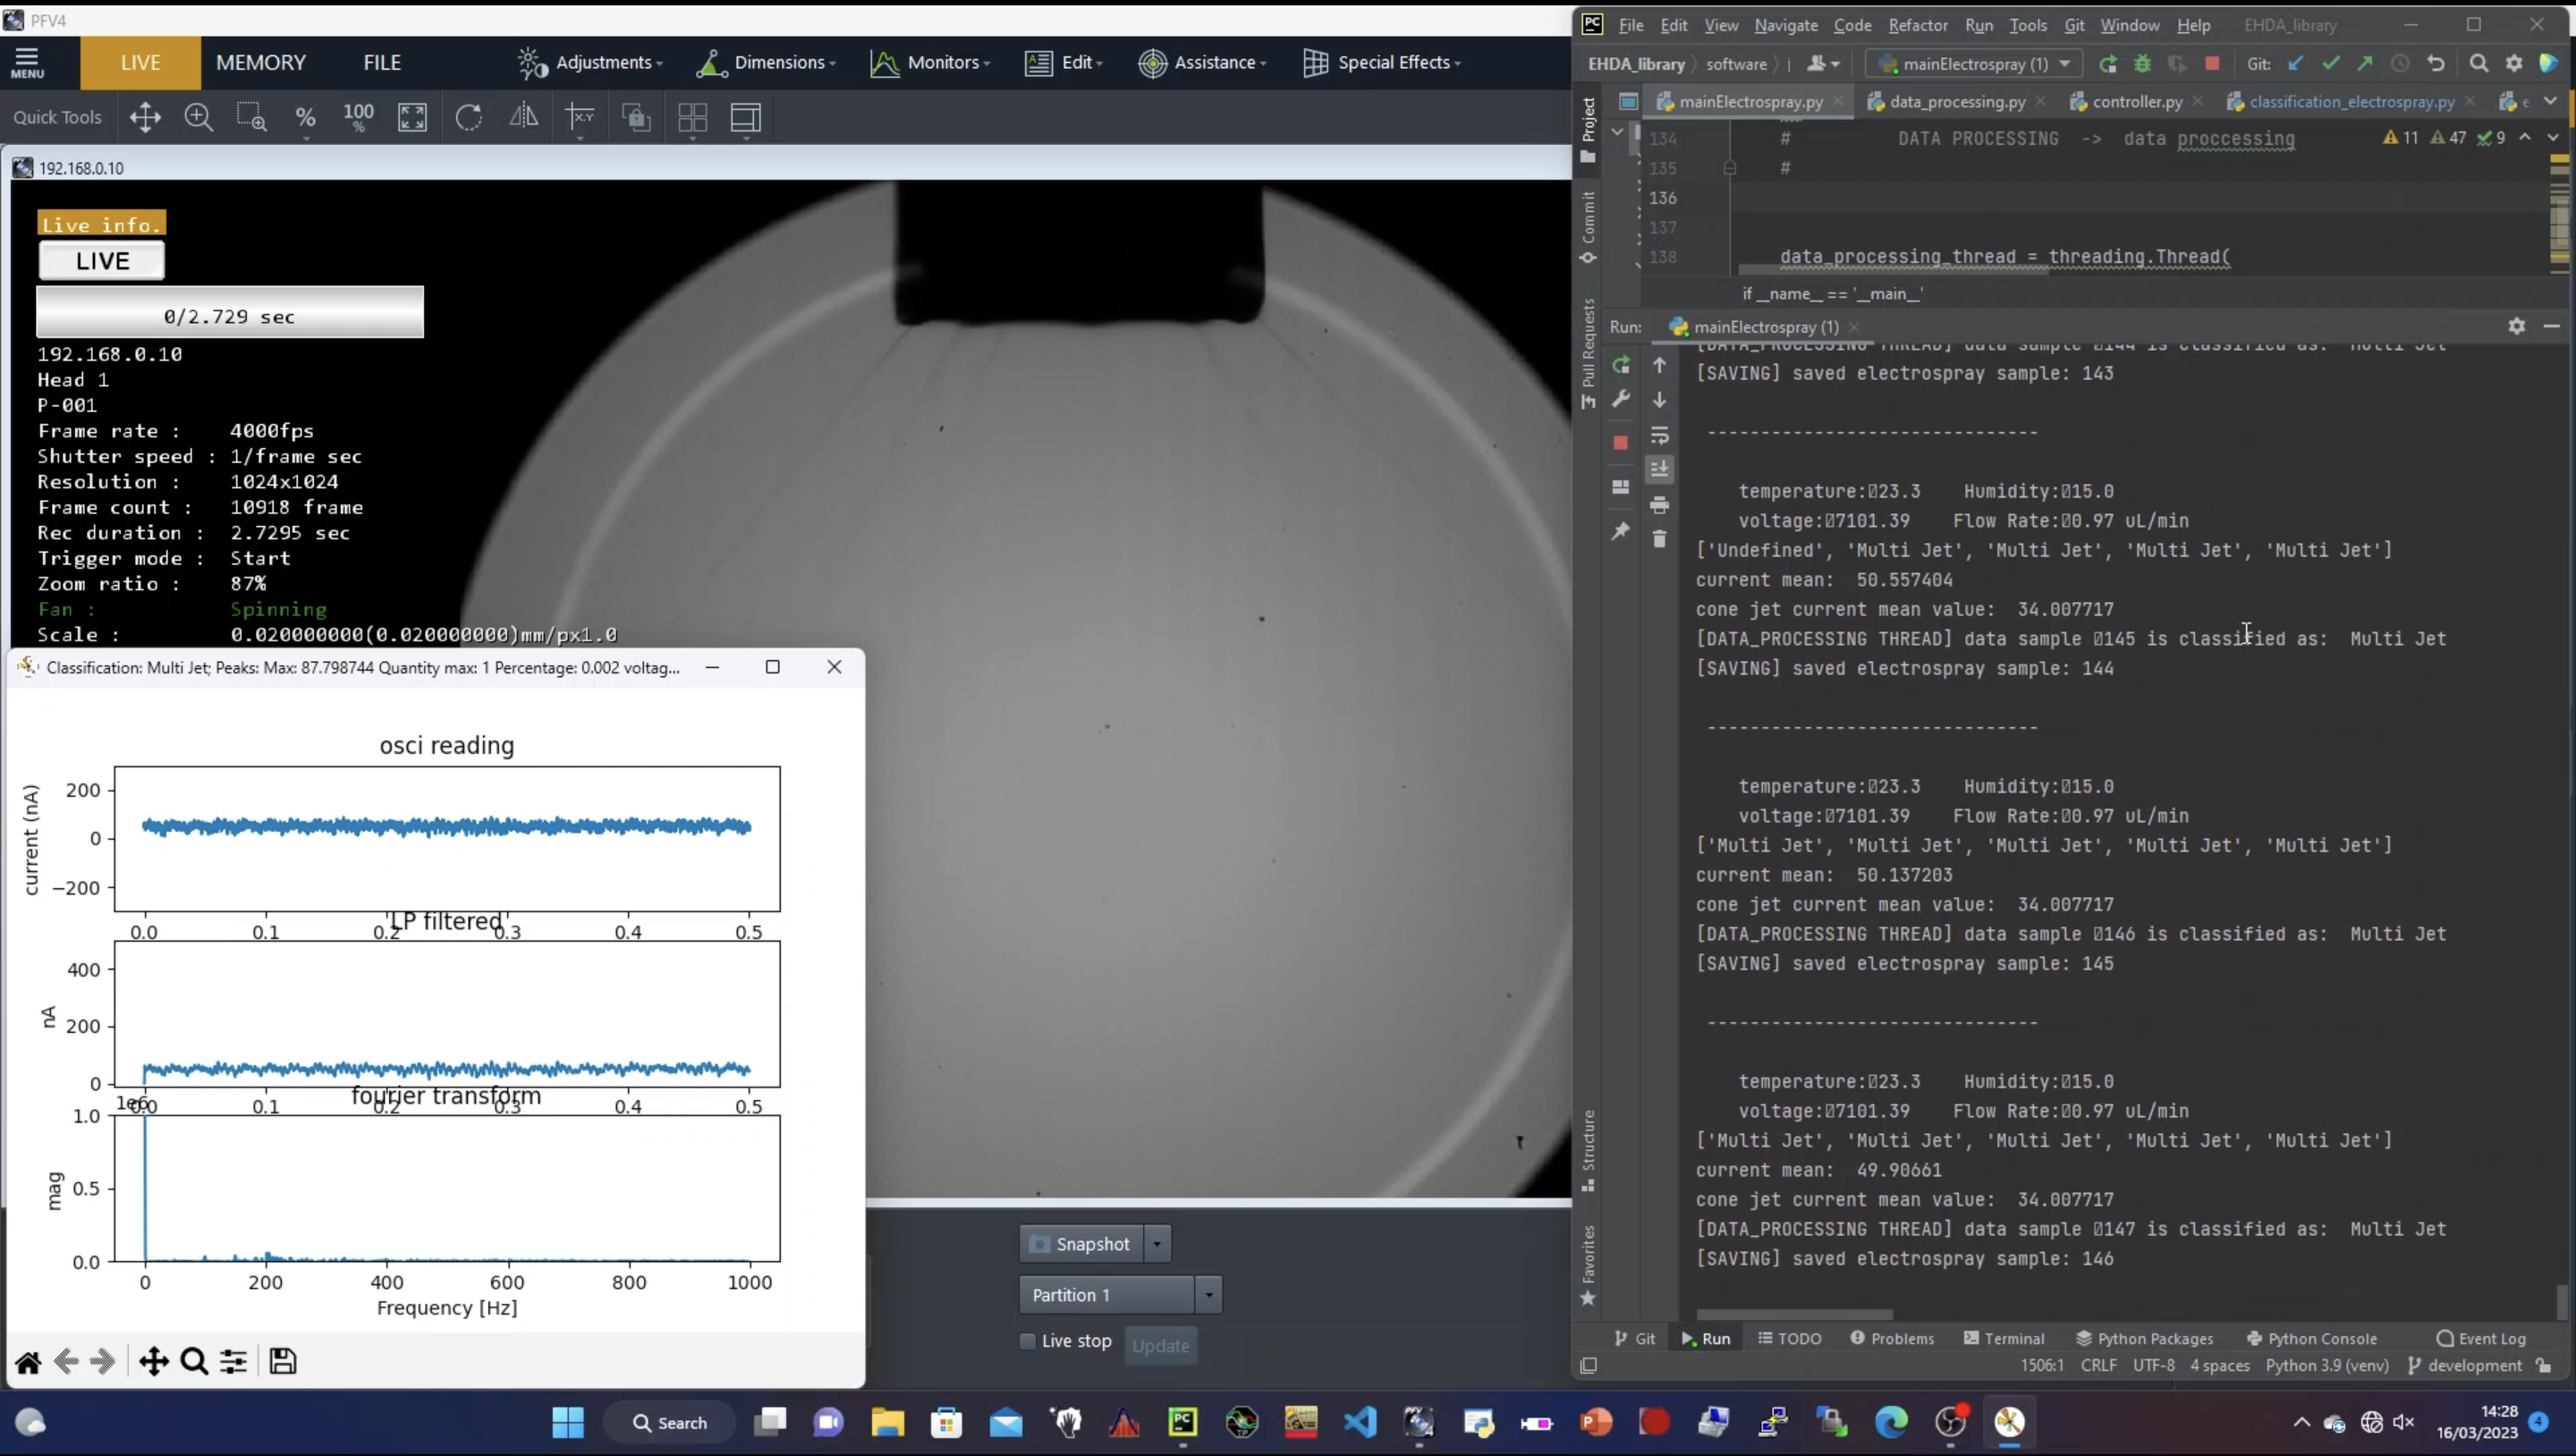
\includegraphics[width=16cm]{Figuras/19:03/axs2.png}}
    \caption{Print screen during an experiment. At this moment we are in Multi Jet spraying mode. At the left we can see the current signal has a smooth and constant curve. We can also see the automatic classification on the right side.}
    \label{fig:multi_class_exp}
\end{figure}


\section{Classification}
\label{sec:classification_results}

The classification results in our algorithm implemented as described in section \ref{sec:section_classification} showed good accuracy for all the classifications described in section \ref{sec:spraying_modes_subsec}.
Nevertheless, the multi jet classification made by a current value factor of 1.14 above the cone jet is just effective for pure ethanol, liquid used in all this project.

Even if the multi jet classification just works for pure ethanol, the data saved with correct classification in ethanol can be used to extract any other signal information about the multi jet or to train a black box classification algorithm.

\subsection{Step Sequence}
\label{subsec:step_results}

Our first classification results were made exploring just the voltage ranges. For that stabilized all the other parameters such as humidity, temperature and external noise.
First, we fixed a flow rate to 0.7 uL/min. and ran a step routine as defined in \ref{subsec:step_routine}. 
The figure \ref{fig:step_voltage} shows the step voltages during the experiment and figure \ref{fig:raw_data} illustrates the raw data acquired with it. 
In figure \ref{fig:class_step_data} we see the same experiment data classified by spraying mode and separated by color.


\begin{figure}[H]
    \center
    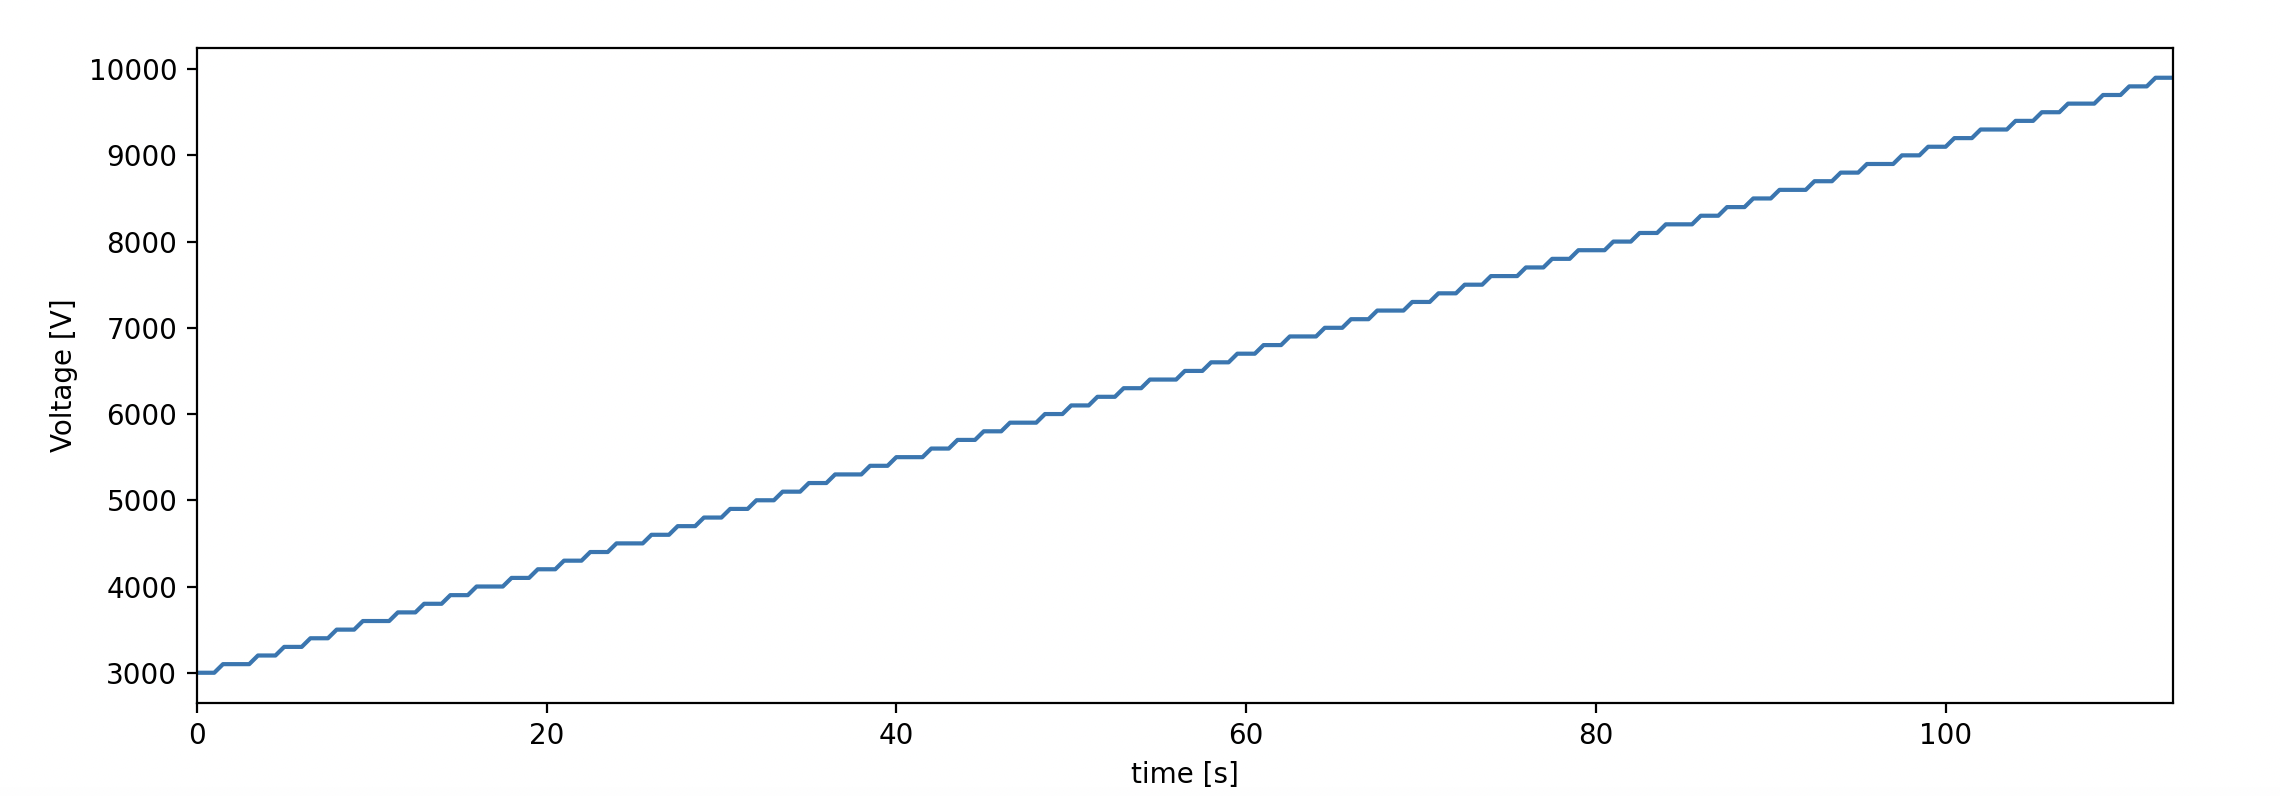
\includegraphics[width=12cm]{Figuras/19:03/voltage_step.png}
    \caption{Input voltage step graph. The range is between 3K-10K Volts. Step size of 50V and step time of 5 seconds.}
    \label{fig:step_voltage}
\end{figure}


\begin{figure}[H]
    \center
    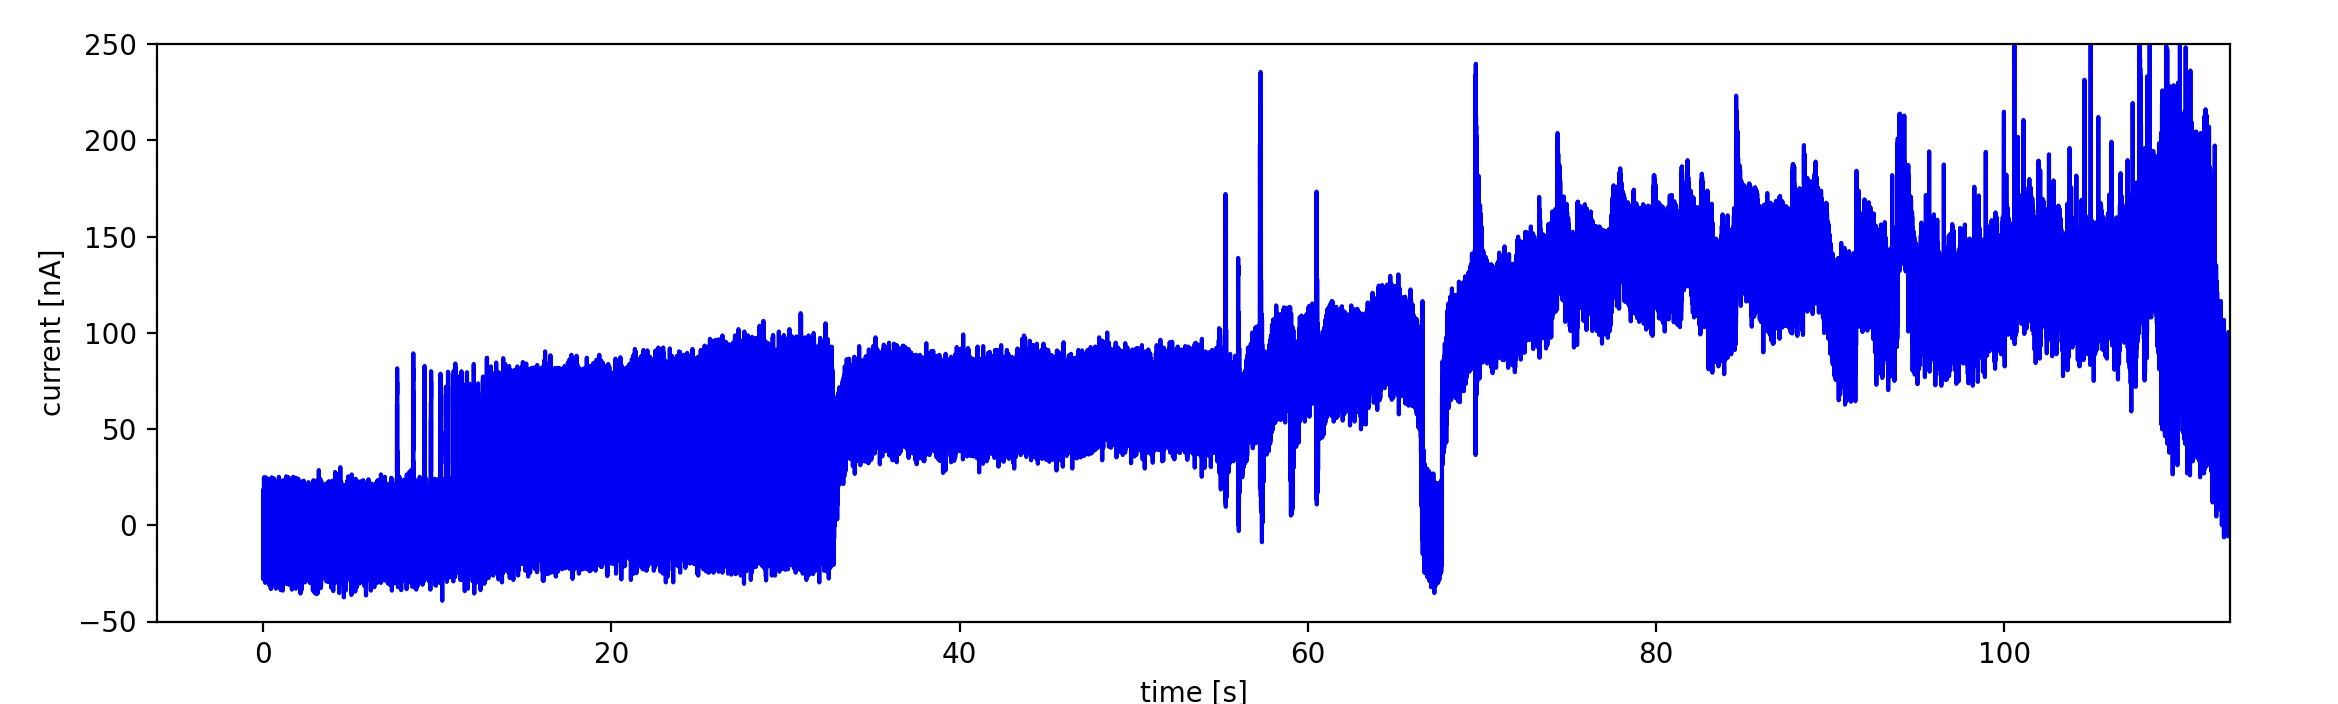
\includegraphics[width=12cm]{Figuras/19:03/raw-data-example.png}
    \caption{Output raw data collected in the voltage range experiment showed in \ref{fig:step_voltage}. The sampling rate of the oscilloscope is 10KHz. This graph has 1.5 Million data points.}
    \label{fig:raw_data}
\end{figure}

\begin{figure}[H]
    \center
    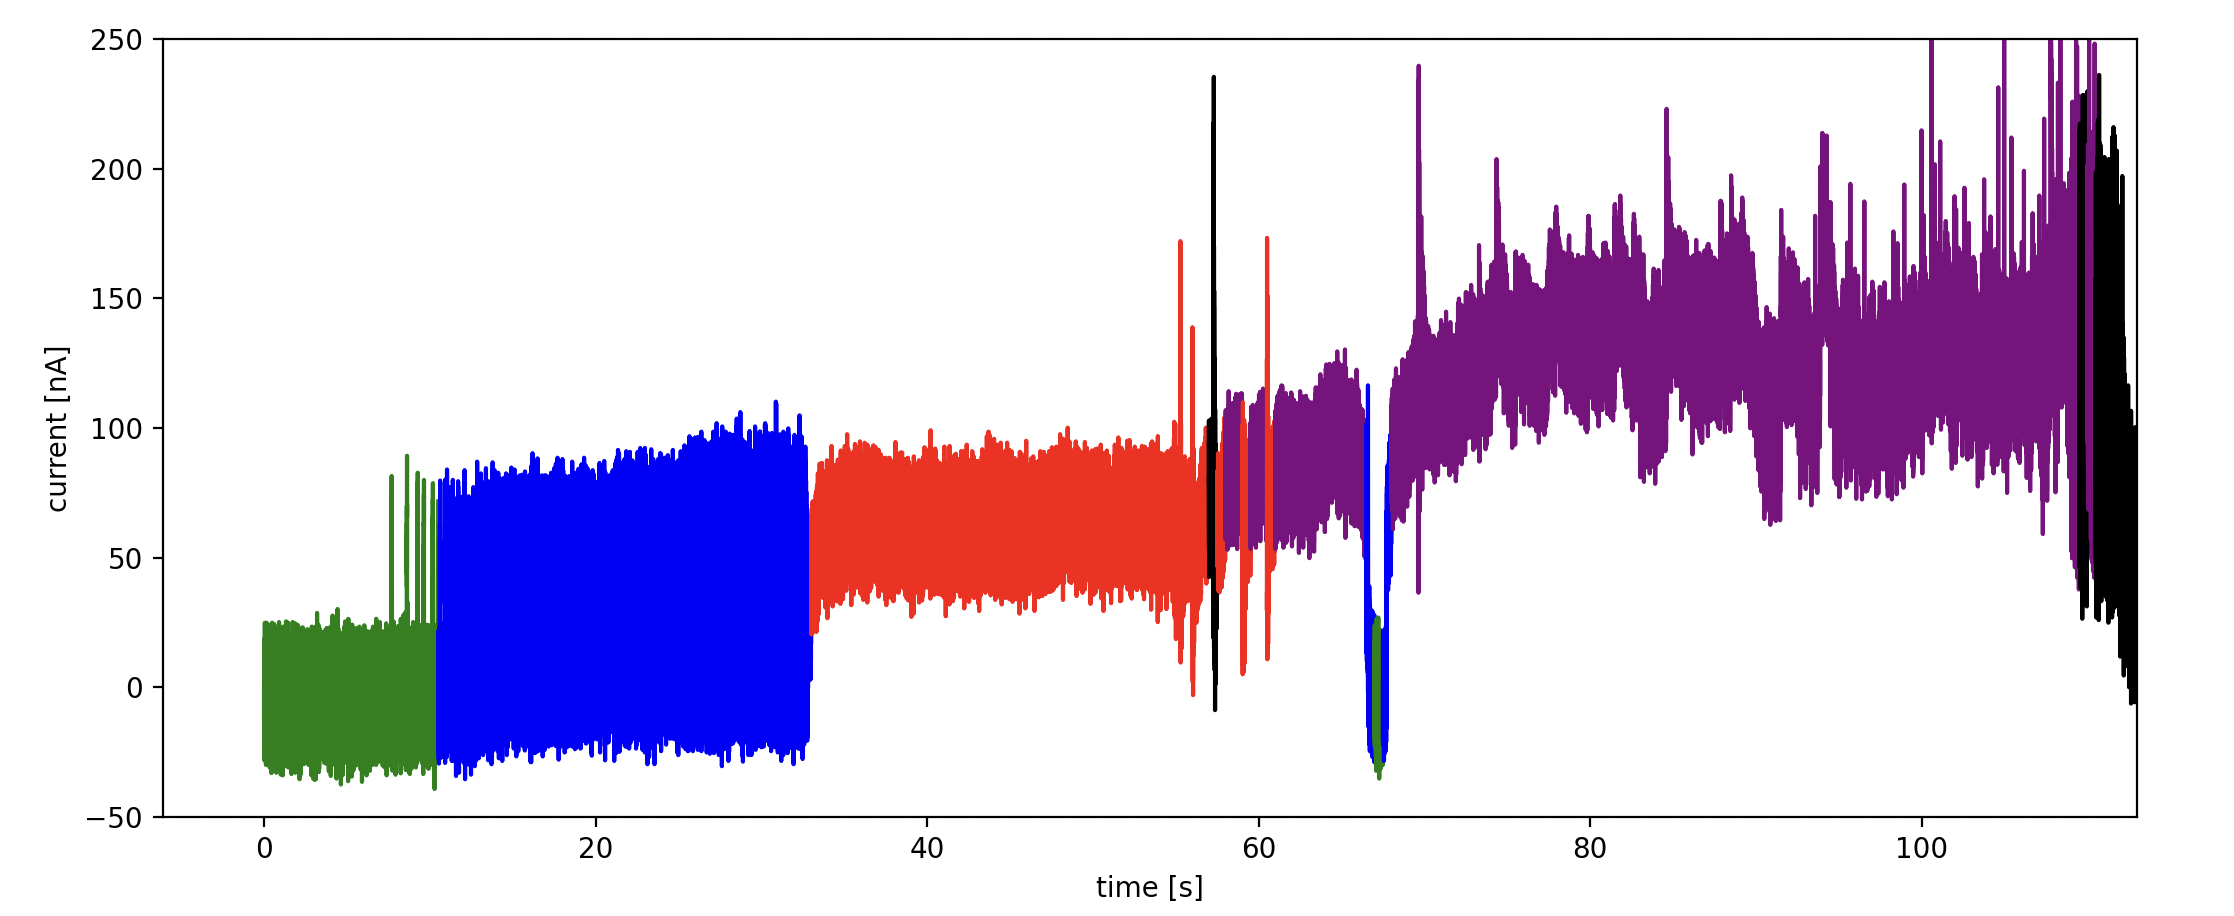
\includegraphics[width=12cm]{Figuras/19:03/classified-data-example.png}
    \caption{The same graph as \ref{fig:raw_data} but after the classification procedure. The colors are green: Dripping, Blue: Intermittent, Red: Cone Jet, Purple: Multi Jet and Black: Undefined.}
    \label{fig:class_step_data}
\end{figure}

The graph of voltage scan as showed in \ref{fig:raw_data} has a common shape for different liquids and parameters. After having familiarity with it is even possible to classify the spraying modes by visual analysis. For example: 
Dripping mode has a current mean of 0V. The Intermittent state has a high variation of values that can be seen by the thickness of the graph. The Cone jet is a thinner graph because the signal is more constant. The Multi Jet is the same as Cone jet graph but with a higher mean value than cone Jet. Corona sparks are not showed in the graph because the discharges has a high current value and will be above the axis limits.



\subsection{Map Sequence}
\label{subsec:map_results}

For validation with literature and also to expose the benefits of the automated routine and classification the map sequence proof itself the best result of this work.



    Firstly, for better understand the spraying dynamics, manual experiments were done.
    Figure \ref{fig:stability_1} shows the stability region of different spraying mode for pure ethanol in the range of voltage and flow rate.

    \begin{figure}[H]
        \center
        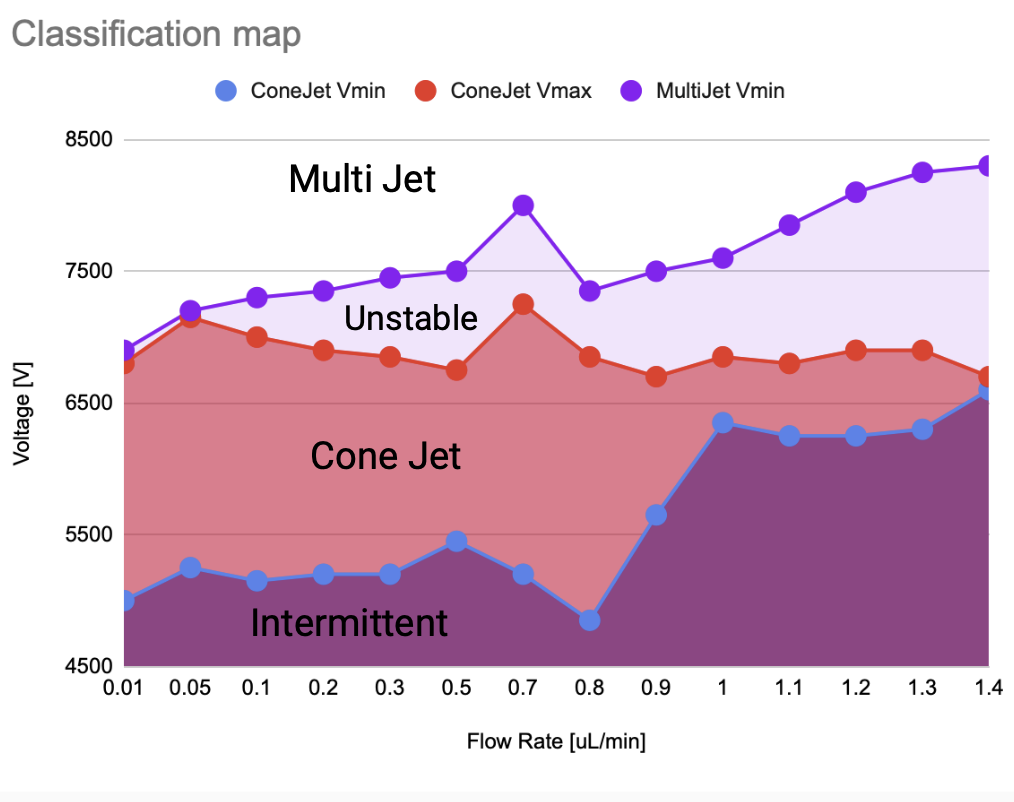
\includegraphics[width=8cm]{Figuras/regions.png}
        \label{fig:stability_1}
        \caption{Spraying modes regions of pure ethanol}
    \end{figure}


    For validation of the automatic classification experiments were made comparing both manual and automatic classification.
    In figures \ref{fig:stability_2} and \ref{fig:stability_3} we can see that the cone jet stability island has a similar shape in both manual (fig. \ref{fig:stability_2}) and automatic (fig. \ref{fig:stability_3}) data collected in the same experiment.

    \begin{multicols}{2}


        \begin{figure}[H]
            \center
            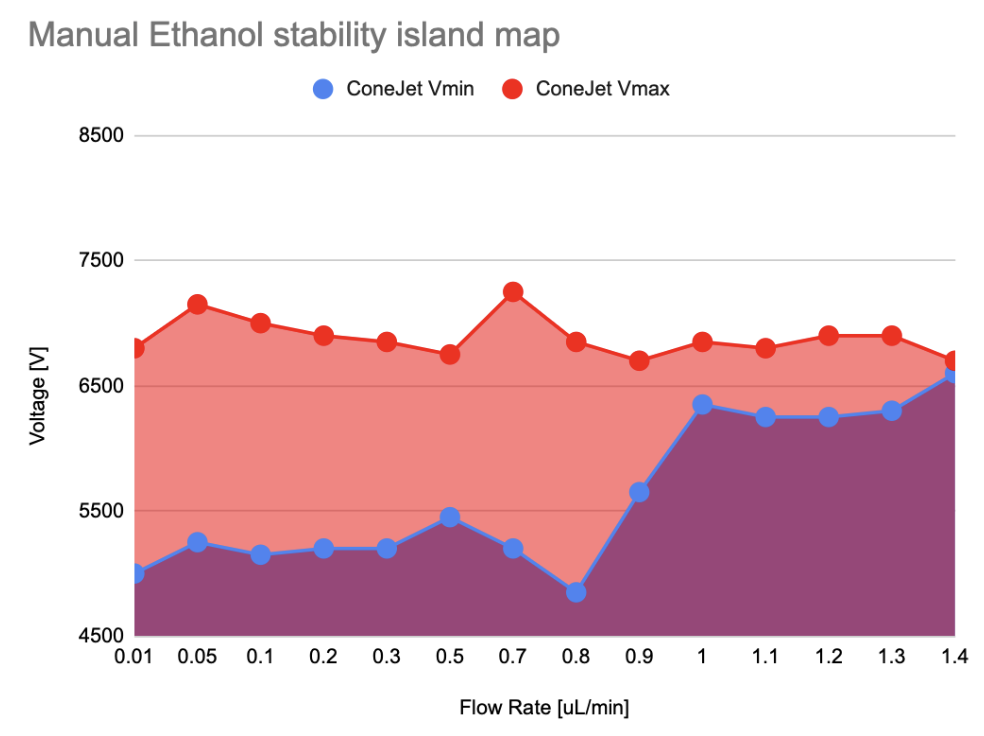
\includegraphics[width=8cm]{Figuras/april/manual_stability.png}
            \caption{Cone jet island manual experiment 1}
            \label{fig:stability_2}
        \end{figure}

        \begin{figure}[H]
            \center
            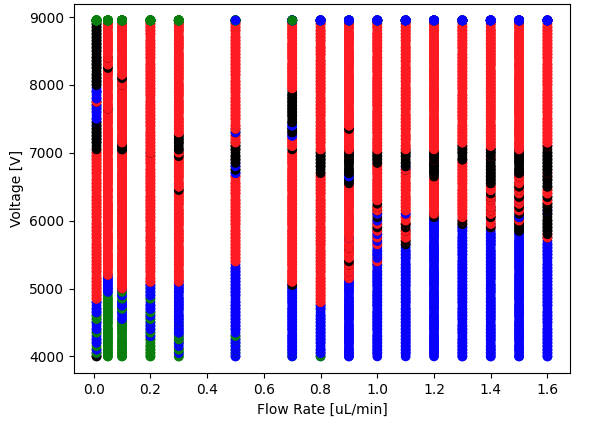
\includegraphics[width=9cm]{Figuras/report3/map-exp-26-01.png}
            \caption{Cone jet island automatic experiment 1}
            \label{fig:stability_3}
        \end{figure}

    \end{multicols}

    We can see in figures \ref{fig:stability_4} and \ref{fig:stability_5} another experiment with the same liquid and a comparison on manual (visually by the high speed camera) and automatic classification.

    \begin{multicols}{2}


        \begin{figure}[H]
            \center
            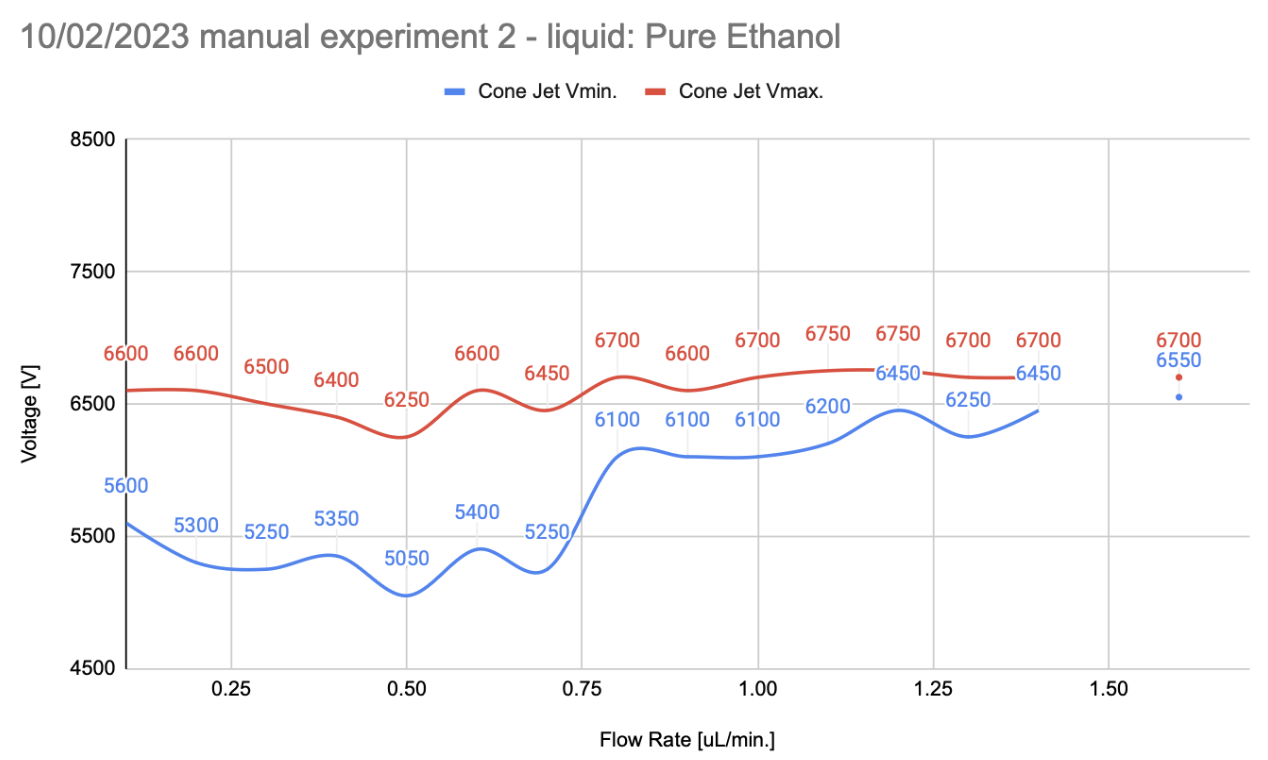
\includegraphics[width=8cm]{Figuras/april/results_map_1.png}
            \caption{Cone jet island manual experiment 2}
            \label{fig:stability_4}
        \end{figure}

        \begin{figure}[H]
            \center
            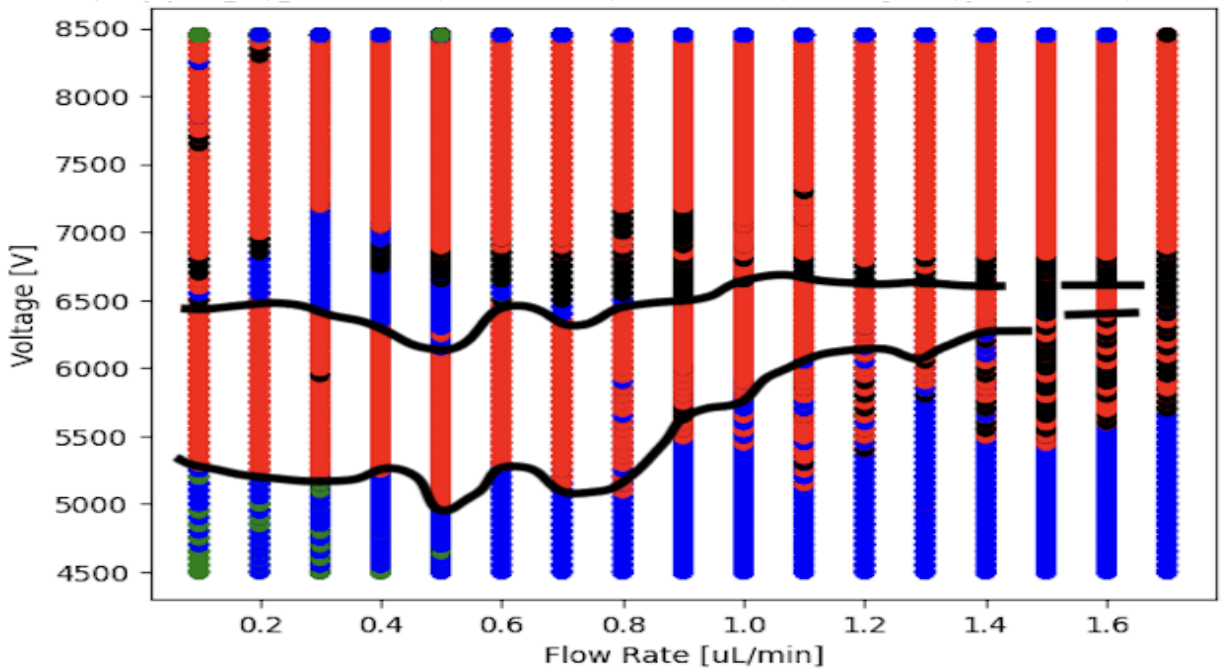
\includegraphics[width=9cm]{Figuras/april/results_map_2.png}
            \caption{Cone jet island automatic experiment 2}
            \label{fig:stability_5}
        \end{figure}

    \end{multicols}

    We can see in figures \ref{fig:stability_6} and \ref{fig:stability_7} the same experiment and results as above, but with the Multi Jet classification that was a new feature in the software.

    \begin{multicols}{2}


        \begin{figure}[H]
            \center
            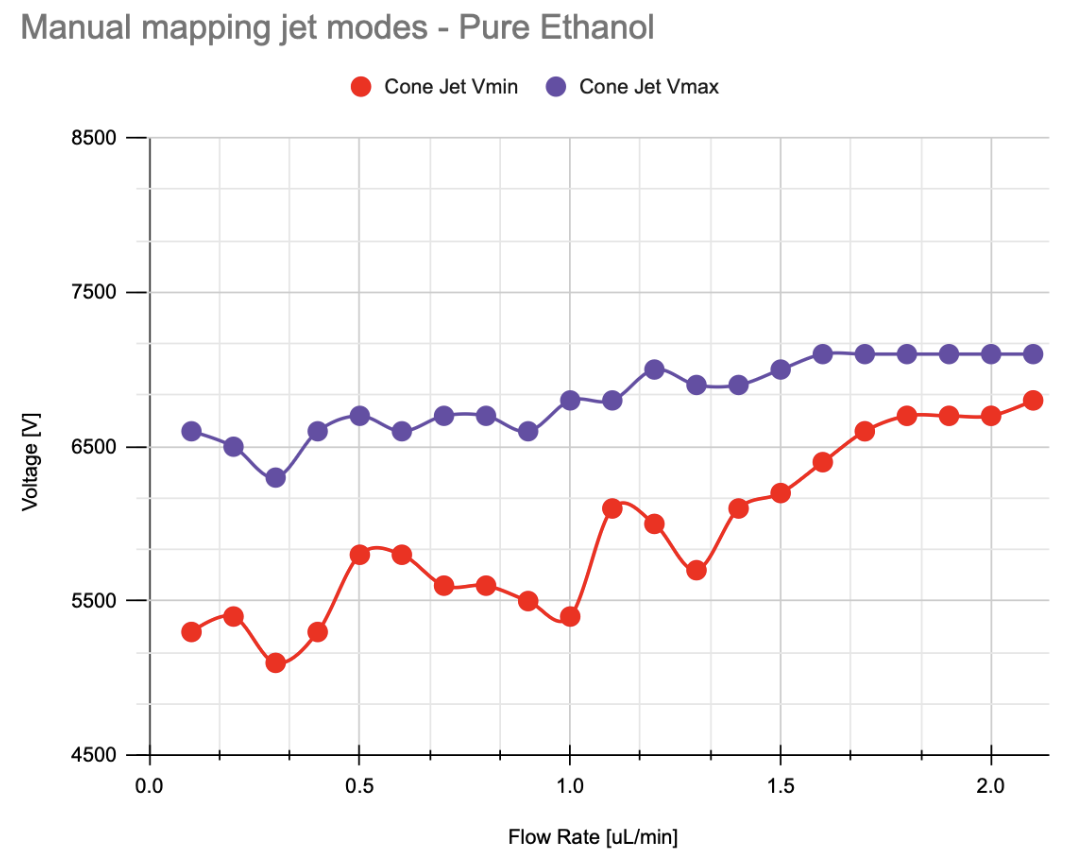
\includegraphics[width=8cm]{Figuras/april/map5.png}
            \caption{Cone jet island manual experiment 3}
            \label{fig:stability_6}
        \end{figure}

        \begin{figure}[H]
            \center
            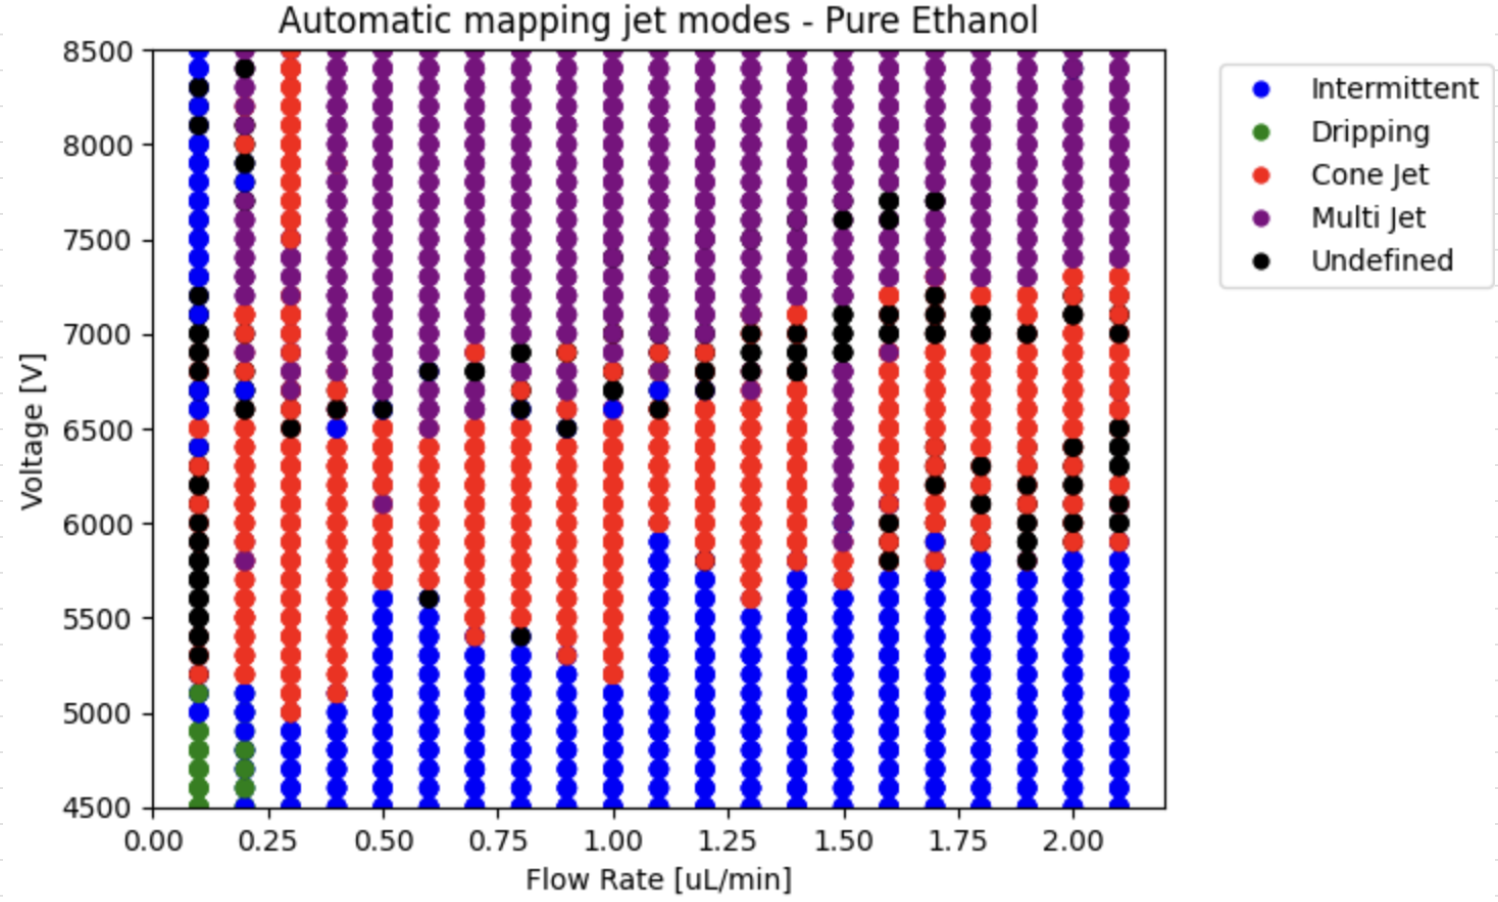
\includegraphics[width=10cm]{Figuras/april/map2.png}
            \caption{Cone jet island automatic experiment 3}
            \label{fig:stability_7}
        \end{figure}


    \end{multicols}

    \vspace{2cm}
    \subsubsection{Non-dimensional axis}


    To compare with the literature and validate the algorithm we decided to display the data using the non-dimensional numbers used in figure \ref{fig:ganan_calvo_fig}.

    \begin{multicols}{2}

        \begin{figure}[H]
            \center
            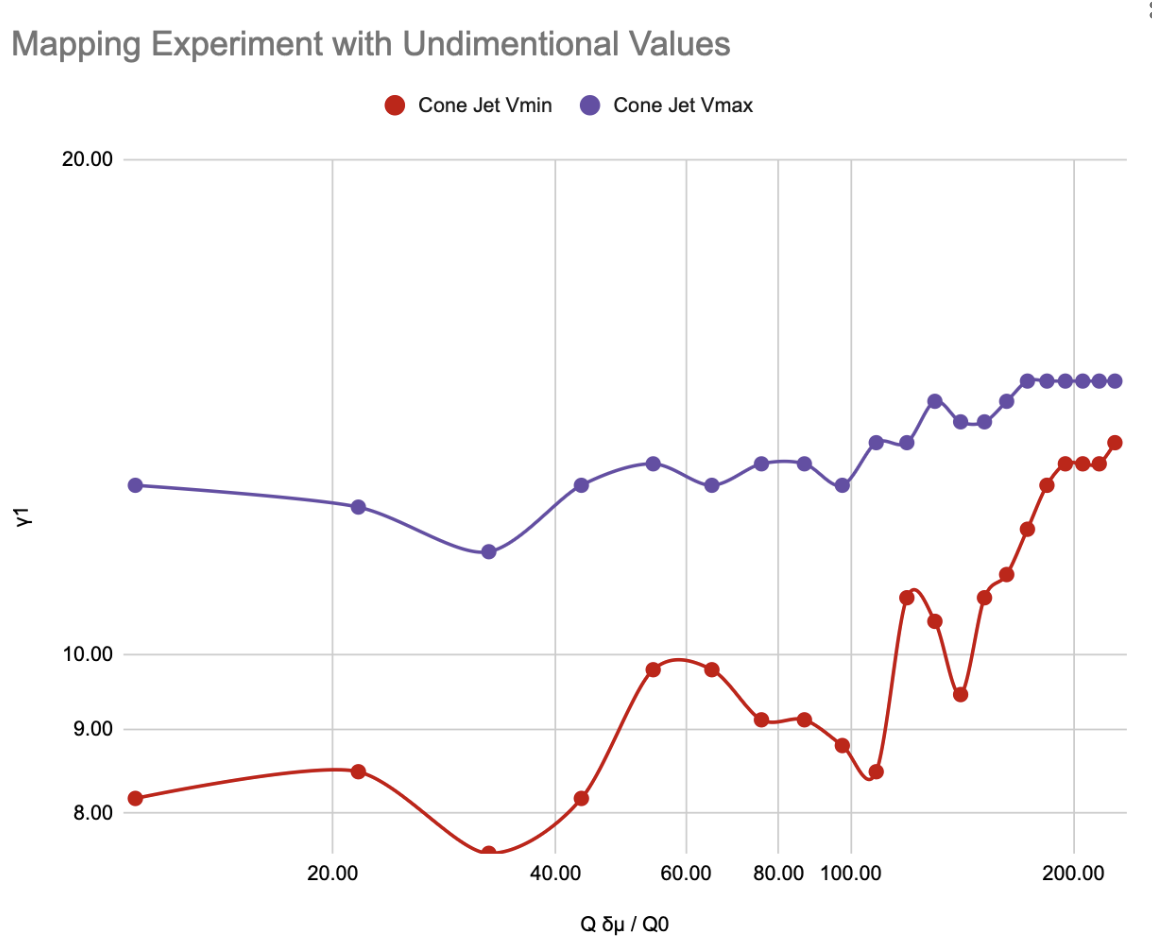
\includegraphics[width=7cm]{Figuras/april/manual_non_dim_exp.png}
            \caption{Cone jet island manual experiment 4}
        \end{figure}

        \begin{figure}[H]
            \center
            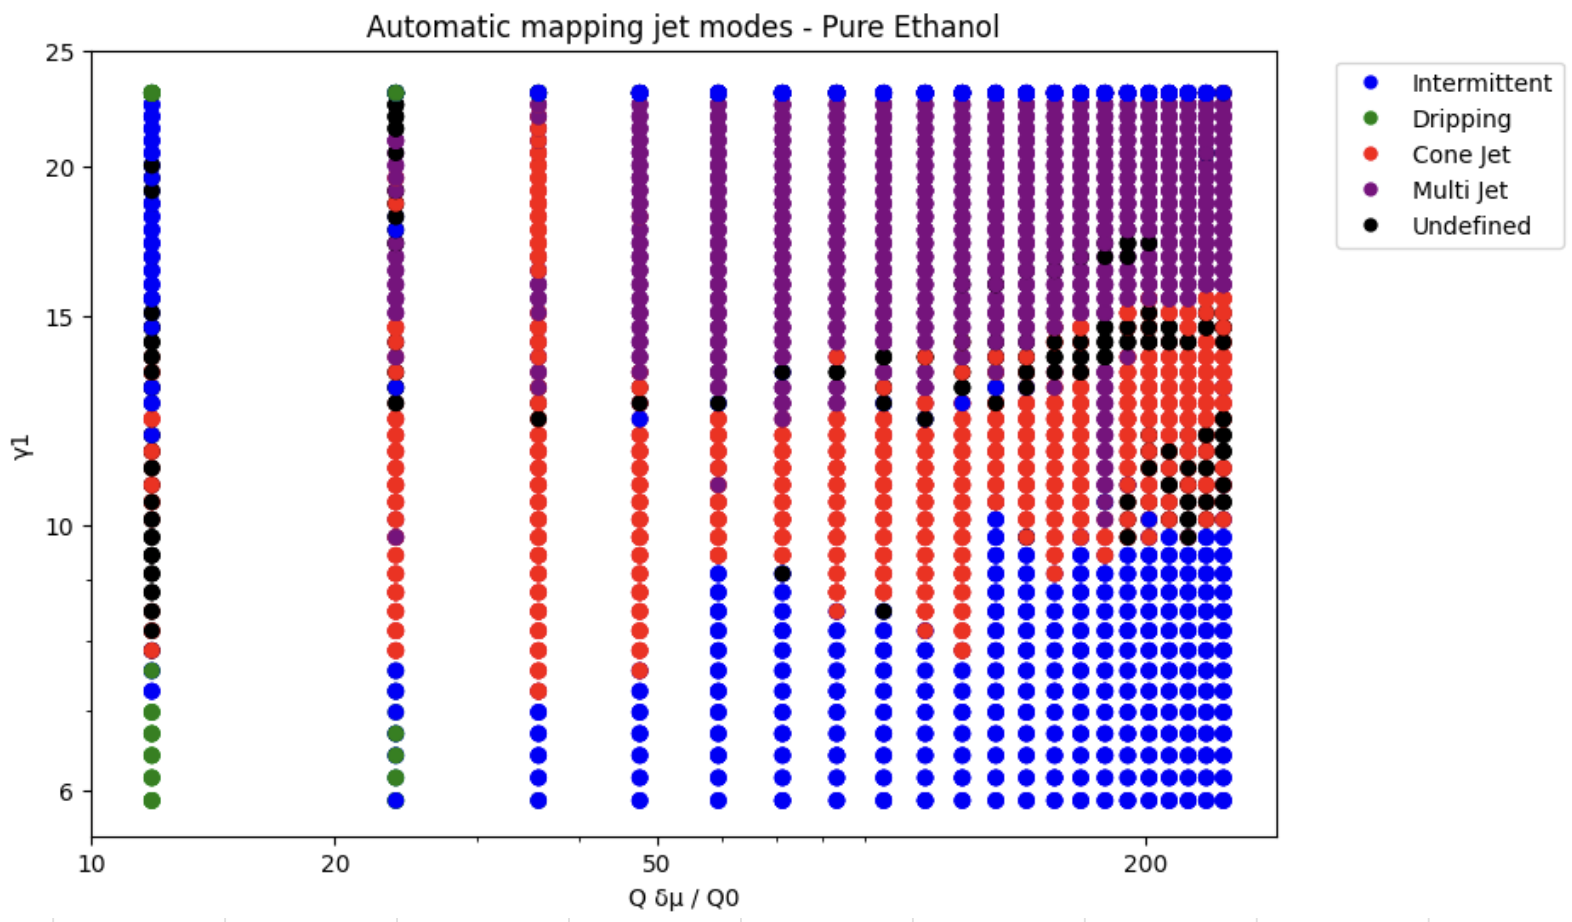
\includegraphics[width=10cm]{Figuras/19:03/non-dimensional-1.png}
            \caption{Cone jet island automatic experiment 4}
        \end{figure}


    \end{multicols}

\section{Controller}
\label{sec:controller_results}

    The results of the classification process were favorable for experiment automation, however, they may not be as effective for optimal performance of the controller.
    The inaccuracy of the classification by statistical method in addition with the amount of variables that need to be syntonized for stabilize in cone jet or multi jet makes it hard to control this process.

    Of particular interest in applications is the cone-jet mode, where the meniscus emits a steady microscopic jet, resulting in uniformly sized droplets. 

        Flow rate perturbation robustness test

        \begin{figure}[H]
            \center
            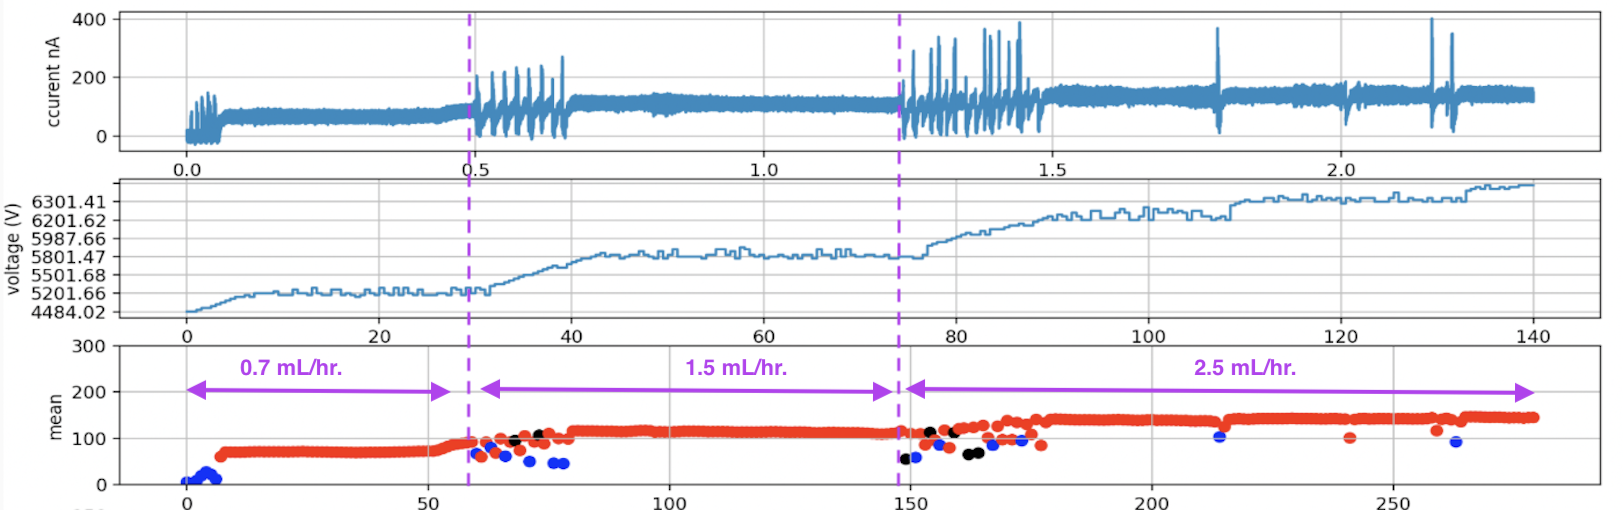
\includegraphics[width=17cm]{Figuras/19:03/control_first_results.png}
            \caption{Simple controller validation experiment. For this experiment we waited the system to stabilize in the desired spraying mode. After that we made a perturbation robustness test changing the flow rate.}
        \end{figure}


\section{Chapter conclusion}


\clearpage